\documentclass{article}

\usepackage[english]{babel}
\usepackage[a4paper,top=2cm,bottom=2cm,left=3cm,right=3cm,marginparwidth=1.75cm]{geometry}

\usepackage{amsmath}
\usepackage{graphicx}
\usepackage{minted}
\usepackage{parskip}
\usepackage{pgfplots}

\usepackage[colorlinks=true, allcolors=blue]{hyperref}

\title{Solving 2048 with Expectimax}
\author{David Cook}

\begin{document}
\maketitle

\tableofcontents
\newpage
\begin{abstract}
The simplest goal of this project is to play the puzzle game 2048 with the expectimax algorithm. I intend to make it able to play any size of the 2048 game, though eventually, any algorithm will break down if the grid is too large. In order to mitigate this, I intend to find ways of pruning the tree as much as possible. Officially the game of 2048 ends when the tile of 2048 finishes however, the game can be continued until no more moves are possible.
\end{abstract}
\section{Introduction}
\label{sec:intro}
\subsection{The Problem}
\label{subsec:problem}
2048 is a game which features a 4x4 grid containing powers of 2. Each game starts with two cells, either 2 or 4.
All the tiles can be slid in any of the four directions simultaneously. When two of the same powers of 2 collide the tiles merge, creating the next power of 2. The new tile increases the score by the value of the new tile. After each move, a new tile (either 2 or 4) will appear on the grid \cite{game2048}.

The goal of this project is to play a 2048 game using an AI-search algorithm. Previous projects have reached the tile of 8192 with reasonable consistency \cite{expectimax2048} but failed to go much higher. Reports were the rules of the game are changed are not very common, so the search algorithm shall play a $n \times m$ game rather than simply the traditional $4 \times 4$ 2048 game.

The most promising search algorithm is expectimax \cite{aiplays2048}. This is an algorithm designed for scenarios where there are two agents, one making random decisions and one making rational decisions \cite[~p.200]{russell2010artificial}. It is not practical to pre-compute a traditional 2048 decision tree, particularly when factoring in variable-size games.

\subsection{Deliverables}
\label{subsec:deliverable}
\subsubsection{Proof of concept programs}
\begin{enumerate}
    \item Decision Tree
    \item Simple Expectimax Example
    \item 2x2 2048 Game
    \item 2048 with a heuristic
\end{enumerate}
\subsubsection{Report}
\begin{enumerate}
    \item Design patterns in AI search.
    \item Techniques used by humans and previous automated solvers.
    \item User interface design for solver
    \item Complexity, NP-hardness and big $O$ notation
    \item The practicality and the effectiveness of the pruning expectimax tree.
    \item The heuristics have been generalised to support more 2048 games.
    \item Describe interesting algorithms and programming techniques, such as expectimax, used in the project.
    \item Implementation and performance of the decision tree.    
\end{enumerate}
The report will describe the implementation and optimisations of the expectimax algorithm, with a focus on any software engineering principles used in the processes. 
\subsubsection{Final Program}
\begin{enumerate}
    \item The final program will be written in java, with a full Object-oriented design, using modern software engineering principles.
    \item Theoretically capable of playing any $nxm$ 2048 game, though eventually break down due to performance.
    \item The program will have a user interface capable of keeping track of stats about the algorithms and an easy way of creating new $nxm$ games.
\end{enumerate}
\section{Proof of Concepts}
\label{sec:proof_of_concepts}
\subsection{Decision Tree}
\label{subsec:dt}
There are many ways of implementing a tree structure; various ones are more appropriate than others. The operations that a required in this situation are \cite{russell2010artificial}:
\begin{itemize}
    \item Generate a tree from the root node.
    \item Transverse the entire tree to calculate the score.
    \item Walk to a direct child node and regenerate the tree. At least the scores will need to regenerate on pre-existing nodes.
\end{itemize}
While this will likely not be true, I will assume generating a node can be done in $O(1)$ time. Generating or traversing nodes in a tree with $n$ nodes, can not be done in any less than $O(n)$. Reading a direct child can not be done in $O(1)$ time. \par
A common approach to making a tree is as follows:
\begin{minted}{java}
public class Node {
    int value;
    Node[] children;
}
\end{minted}
This is a node with an array of references to its child nodes. Traversing this entire tree will have a time complexity of 
$O(n)$. Arranging these nodes into a tree structure takes $O(n)$ and finally picking a direct child of a node takes $O(1)$,
Therefore there is no need to pick a less common tree implementation.

\subsection{Expectimax}
\label{subsec:expectimax}
\begin{figure}
    \centering
    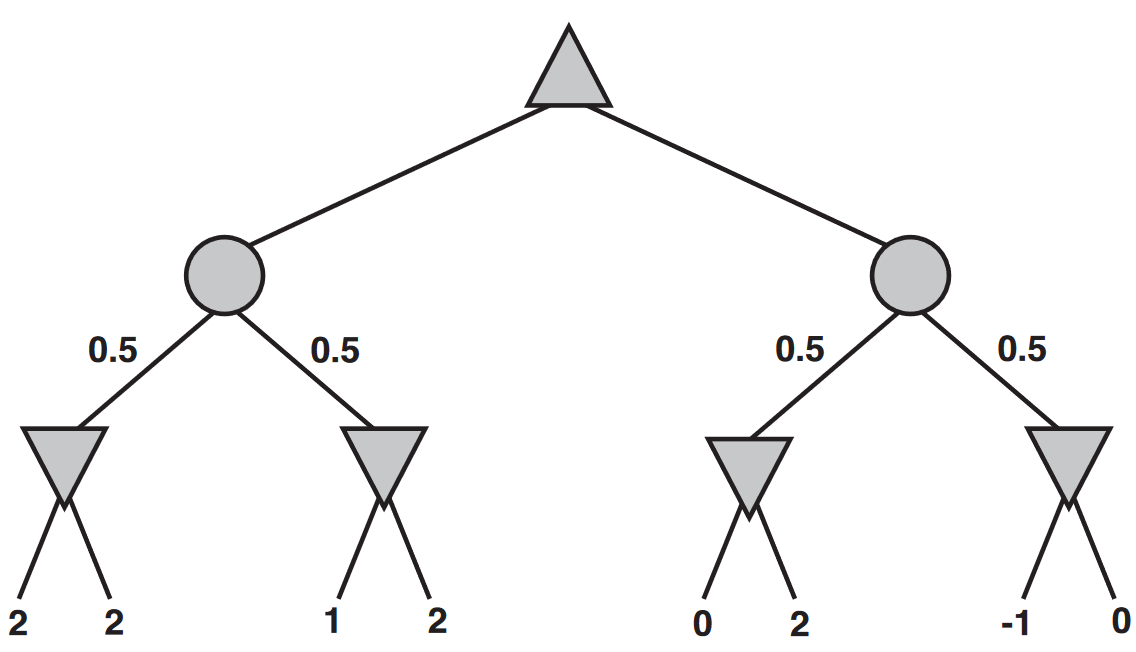
\includegraphics[width=0.7\textwidth]{expectimax.png}
    \caption{An image of an expectimax tree \cite[p.~200]{russell2010artificial}}
    \label{fig:expectree}
\end{figure}
The decision tree required in the expectimax algorithm (Figure \ref{fig:expectree}) has three types of nodes, however, only two types of nodes are needed for the problem of solving 2048. These three types of nodes include:
\begin{itemize}
    \item Maximising nodes: These nodes get the maximum scoring child of the node, and acquire the same score
    \item Chance Nodes: These nodes represent situations where there are random states that may follow. The link weights between
    a chance node and its children represent the probability of that event occurring.
    \item Minimising Nodes: These are the opposite of maximising nodes, I do not expect to need them in this project.
    \item Terminus nodes: These nodes are the leaves of the tree. Their score is already known and used to calculate the score in the rest of the tree.
\end{itemize}
Each of these three relevant types of nodes has been converted to individual java classes, storing the scores in a float

attribute. This means that the value of the score only needs to be retrieved once.

\subsection{2048}
\label{subsec:2048}
This proof of concept was created mostly using one source \cite{source2048}, the original 2048 source code. While I did not
directly copy any of the code I read through most of the code relevant to the key features of the game and tried to understand 
why things were done that way. I then re-wrote the code in java using similar approaches.

I learnt a few things that were very useful while writing this prototype. For example: 
\begin{itemize}
    \item If you loop over the numbers in the wrong order a tile may collide with a tile that will be moved later. 
    See Figure \ref{fig:slidebug} for an example.
    \begin{figure}
        \centering
        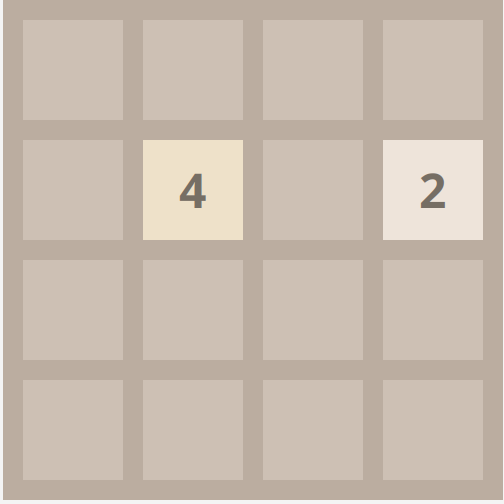
\includegraphics[width=0.3\textwidth]{2048_slide.png}
        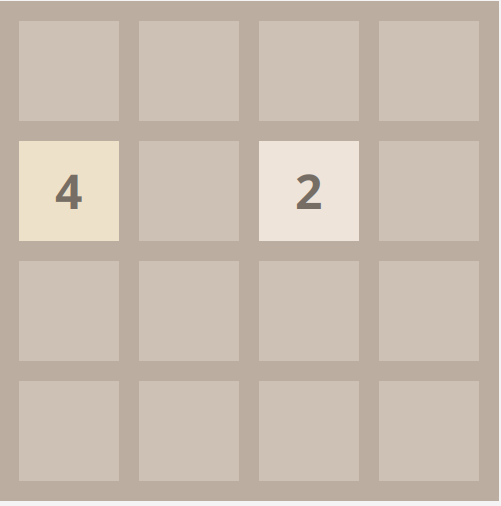
\includegraphics[width=0.3\textwidth]{2048_slide2.png}
        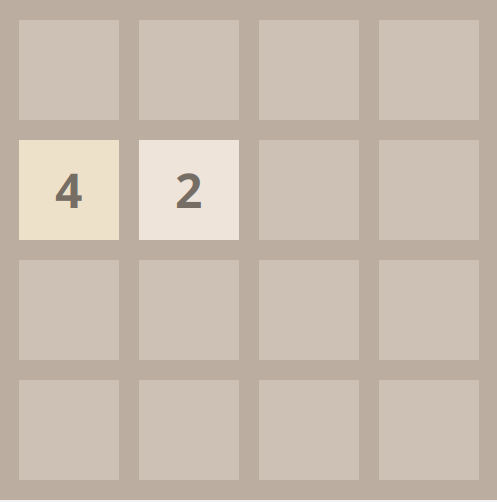
\includegraphics[width=0.3\textwidth]{2048_slide3.png}
        \caption{The first image shows a state where the bug can occur, second shows the bug, third shows what should happen}
        \label{fig:slidebug}
    \end{figure}
    \item When merging tiles, you need to ensure that you do not merge a tile multiple times. See Figure \ref{fig:mergebug} for an example.
    \begin{figure}
        \centering
        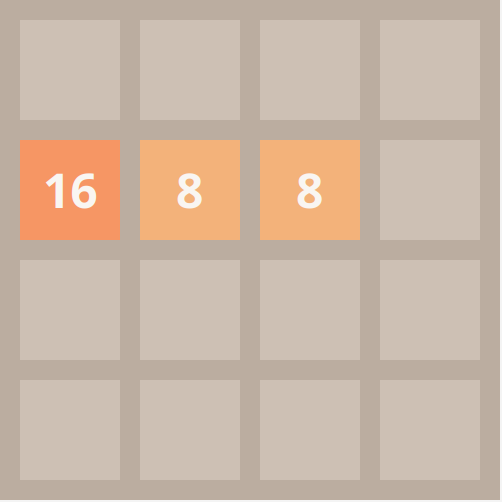
\includegraphics[width=0.3\textwidth]{2048_merge.png}
        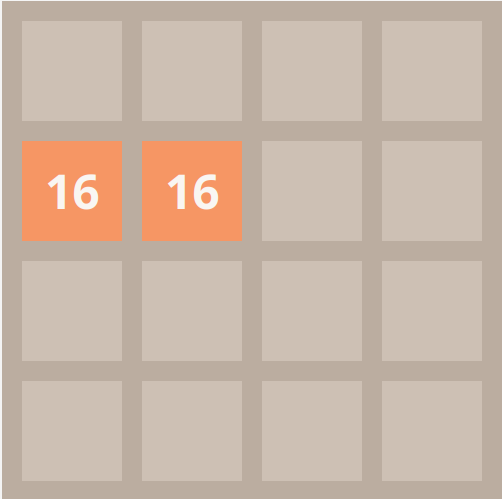
\includegraphics[width=0.3\textwidth]{2048_merge2.png}
        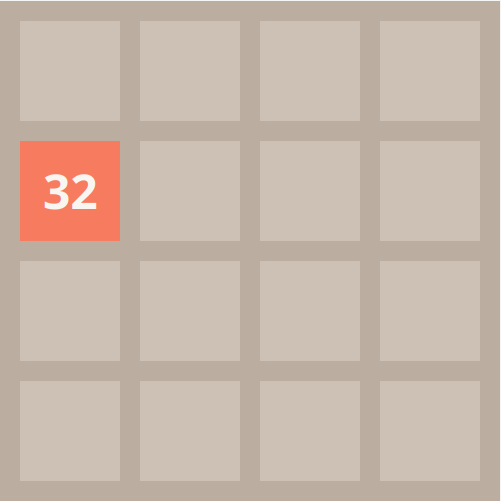
\includegraphics[width=0.3\textwidth]{2048_merge3.png}
        \caption{The first image shows a state where the bug can occur, second shows what should happen, third shows what happened after the bug occurs}
        \label{fig:mergebug}
    \end{figure}
\end{itemize}
The first bug was one that I was expecting to have to test for. However, I had not thought of the second case before writing the proof of concept. I only caught the second bug because I wrote a simple interface allowing me to play the game and pick up on bugs.
\subsection{2048 with Expectimax}
\label{subsec:2048_expectimax}
The expectimax algorithm is working, and there is a working of a 2048 game. These components need to be modified so that the expectimax algorithm can be applied to 2048 specifically. 
I want to generate the full tree instead of using a heuristic, but in order to do this, the 2048 puzzle must be simplified.

Two modifications were made to the setup of 2048 to ensure the tree was a reasonable size:
\begin{itemize}
    \item Make the game $2 \times 2$.
    \item After a move, only the number 2 can appear.
\end{itemize}
With these modifications, there are at most only three possible free cells where a tile can be added. With possible moves, the tree can only grow by $3 \times 4 = 12$ for each move.
A traditional 2048 game has four possible moves and 15 possible free cells where a tile can be added, meaning the tree can grow by $15 \times 4 = 60$ for each move.

Originally the only modification to the game was making it $2 \times 2$ to increase the tree by $6 \times 4 = 24$ for each move. However, the prototype was unable to calculate the tree within a reasonable amount of time.
\subsection{Heuristic for 2048}
\label{subsec:heuristic}
In this prototype, the restrictions were removed from the game. The size of the game is now $n x m$, and either a $2$ or $4$ can appear in the grid. This makes it impracticable to calculate the full tree. To do this, an arbitrary  depth limit is chosen for the tree. At the leaf nodes in the tree, a heuristic value is calculated. 

The first implementation of this prototype was made with a simple heuristic value.
\begin{itemize}
    \item Sum up all the items in the grid. This was a simple heuristic to ensure that the algorithm worked as expected. This heuristic was not very effective.
    \item Sum up all the values multiplied by the row they are in (Top row = 1 and bottom row = n). If this prototype works as expected, the most rewarding path should place larger numbers lower in the grid. Witnessing this effect proved that my algorithm was making good decisions based on the heuristic. This heuristic was much more effective, reaching a tile of 512.
\end{itemize}

With this, the algorithm can theoretically be applied to any 2048 game, which becomes impractical for a large $depth, n$ or $m$. The original plan was to apply this to a 2x2 game, however, due to the nature of the heuristics, I removed this requirement.
\section{User Interface Design}
\label{sec:ui}
\begin{figure}
    \centering
    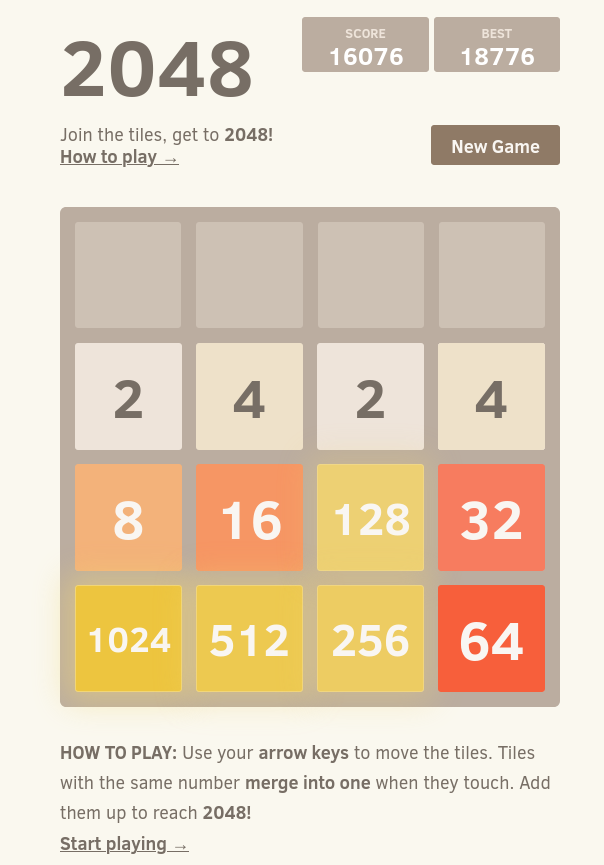
\includegraphics[width=0.4\textwidth]{2048-interface.png}
    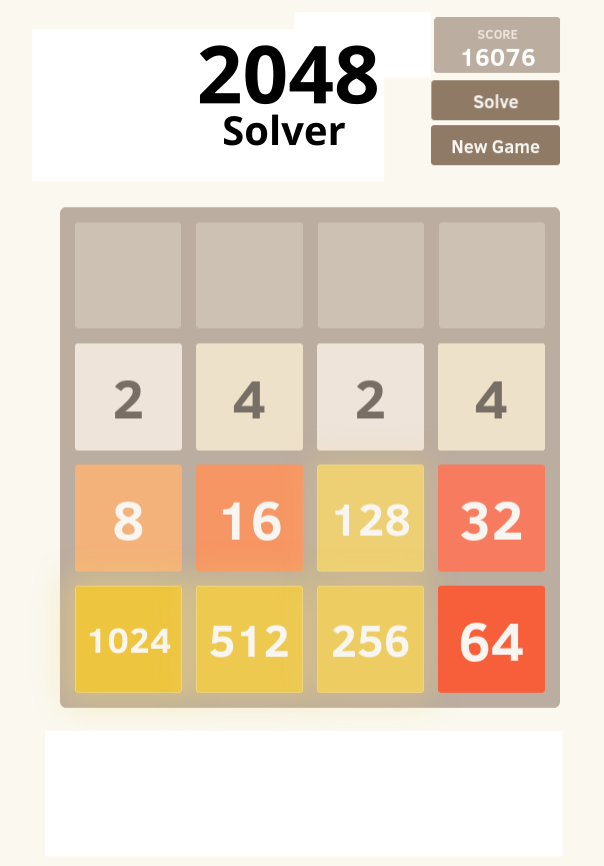
\includegraphics[width=0.4\textwidth]{interface-mockup.png}
    \caption{On the left is a screenshot of the official 2048 user interface \cite{game2048} and on the right
    is an edited version of this image designed to represent what my main interface might look like}
    \label{fig:2048interface}
\end{figure}
I would like the user interface to  resemble the original 2048 game, which can be seen in Figure. \ref{fig:2048interface}.
Parts of the user interface are appropriate for my solver. However, some features need to be removed, and other parts will need to be removed.

Firstly the instructions on how to play the game seen at both the top and bottom of the page can be removed
as the game will play itself. This means there will need to be a new solve button will need to be added.

I will also likely remove the 'best' score box from the interface. I will need to keep track of more data than the best score to evaluate how effective the algorithm is and will likely log this in a CSV file instead.

When the new game button is clicked, I will ask the user how big to make the game. This will be done with a dialogue asking the user how big the game is. When the gird is resized I will also change the minimum size of the window to ensure there is enough space for the game to be readable.

Most versions of 2048 have an animation that plays as the tiles slide; while this would be possible, as animations do exist in JavaFX \cite{javadocfx} however, I am not familiar with them, and think it is not worth the time to re-implementing the animations.

When creating a new game, it is important that the user can enter the size of the new game; however, this input should not be visible when the user doesn't want to make a new game. A long-established solution to this is providing the user with a popup dialogue asking for the size of the game. There is no reference for this in the original 2048 to base the user interface on, so instead of modelling an existing interface, I have created a mock-up of what the interface should look like figure \ref{fig:popup}.

\begin{figure}
    \centering
    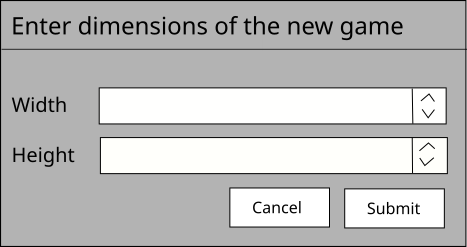
\includegraphics[width=0.4\textwidth]{newGamePopup.png}
    \caption{Mock up of the new game popup window.}
    \label{fig:popup}
\end{figure}
\section{Design Patterns for AI Search}
\label{sec:dp}

\section{Techniques used to solve the game}
\label{sec:techniques}

\subsection{Human Approaches}
\label{subsec:human_techniques}
It can be very difficult to automate a human strategy however it is possible to reward or penalise certain states, and human strategies can be a good place to start when looking for features to reward or penalise.

One human strategy is to keep the largest number in a corner and have a gradient leading to the smaller values like in figure \ref{fig:gradient}\cite{strategy2048}. In testing, it was found this way of arranging the grid makes it relatively easy to merge multiple tiles together in a few moves and reduces the risk of trapped values. However, it does lead to many duplicate values that are difficult to merge, which means there is often not enough space to reach the larger tiles.
\
\begin{figure}[!tbp]
    \centering
    \begin{minipage}[b]{0.45\textwidth}
        \centering
        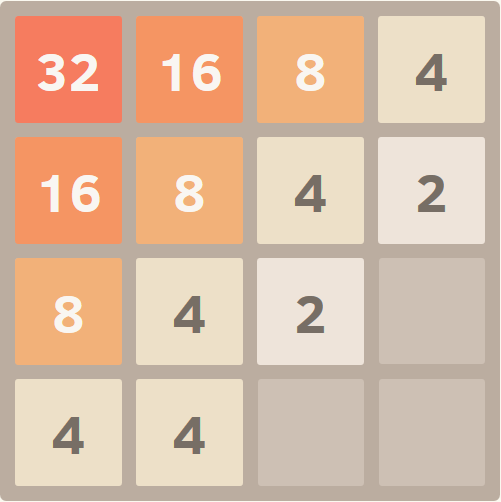
\includegraphics[width=0.5\textwidth]{gradient.png}
        \caption{Gradient pattern used in a 2048 human strategy \cite{strategy2048}.}
        \label{fig:gradient}
    \end{minipage}
    \hfill
    \begin{minipage}[b]{0.45\textwidth}
        \centering
        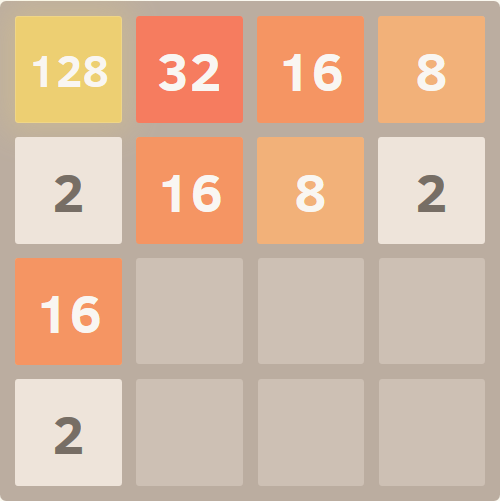
\includegraphics[width=0.5\textwidth]{trapped.png}
        \caption{Example of a trapped value in 2048 \cite{strategy2048}.}
        \label{fig:trap}
    \end{minipage}
\end{figure}
A trapped value is a value surrounded by larger numbers \cite{strategy2048}, such as the 2 in \ref{fig:trap}. Partially when there are not very many free cells around, these cells can be very difficult to get rid of and can take up useful space. They often appear when an empty tile is created after a merge in an area with large numbers. 

Another approach is to try and order the tiles into ascending order using a snake shape \cite{aiplays2048}. The source for this approach describes an automated approach; however,
humans can also use this. In testing, this was found to be the best a very reliable strategy, even reaching tile 8192. The main drawback of this approach was that when merging the row with the largest numbers, it was a risk of producing a trapped value. With careful planning and some luck, it is possible to recover from these states.
\subsection{Automated Approaches}
\label{subsec:automated_techniques}
Many algorithms can be used to solve 2048, to varying degrees of success. Some of these algorithms are \cite{approches2048}:
\begin{itemize}
    \item Minimax - assumes that two rational agents always make their most optimal move \cite{minmaxCS2910}, this strategy does not adapt very well to 2048, according to \cite{approches2048} when citing \cite{minmax2048}.
    \item Expectimax - This is a much more effective strategy, it is similar to Minimax; however, the second agent will always make random decisions \cite[p.~200]{russell2010artificial}. This model lends itself much better to 2048 \cite{expectimax2048}.
    \item Monte-Carlo Tree-Search - "Produces asymmetric trees, effectively pruning poor paths allowing for deeper searching on paths with greater potential." \cite{approches2048}. This method was highly effective compared to Mini-max and Expectimax.
    \item Average Depth-Limited Search - "ADLS approximates expectimax by running multiple simulations, it does not try to calculate all possibilities. Instead, likely outcomes will repeat more often." \cite {approches2048}. This method was highly effective.
\end{itemize}
While there are many different algorithms, and some can be very effective, this report will focus on the expectimax algorithm. This is a relatively simple but effective algorithm \cite{expectimax2048}. The proof of concept program described in section \ref{subsec:2048_expectimax} calculates an entire tree for a $2\times2$ 2048 game. In order to make this practical, I made it so that all new cells had a value of $2$; otherwise, the tree was too large to calculate. For a traditional 2048 game, there are even more possibilities, leading to an even bigger complete expectimax tree. Previous projects have used a depth-limited expectimax tree \cite{aiplays2048}, sometimes even with a dynamic depth \cite{expectimax2048}.

To evaluate how good a state at the end of the tree is, a heuristic function is needed. Two interesting heuristics will be covered in this section. 

\subsubsection{Snake Heuristic}
\label{subsec:snake}
The snake heuristic is based on the most effective heuristic in \cite{aiplays2048}.

This heuristic works by calculating a weighted sum of the values in the grid like this:
\[
    \text{Let }S\text{ be the state of the game, }W=\begin{bmatrix}
    4^{15}&4^{14}&4^{13}&4^{12}\\
    4^8&4^9&4^{10}&4^{11}\\
    4^7&4^6&4^5&4^4\\
    4^0&4^1&4^2&4^3
    \end{bmatrix} \]\[\text{and }h(S)\text{ be the heuristic function.}
\]\[
    h_1(S)=\sum_{i=1}^{4}\sum_{j=1}^{4}W_{i j}S_{i j}
\]

This heuristic takes the human strategy of organising into snake shape rewards boards where this strategy has been applied.
\subsubsection{Diagonal Heuristic}
The diagonal heuristic is used in the project \cite{expectimax2048}.
Similar to the snake heuristic, part of this is a weighted sum. However, there is also a penalty.

The penalty function $p(i, j) = \sum |\text{difference between each neighbour}|$. 

The heuristic function, where $S$ is the games state, and
$
W=\begin{bmatrix}
    6&5&4&1\\
    5&4&1&0\\
    4&1&0&-1\\
    1&0&-1& -2\\
\end{bmatrix}
$ is:
\[
    h_2(S)=\sum_{i=1}^{4}\sum_{j=1}^{4}W_{ij}S_{ij}^2 - \sum_{i=1}^{4}\sum_{j=1}^{4}p(i,j)
\]

\subsubsection{Compassion between Snake and Diagonal Heuristics}
After implementing these heuristics, the maximum tiles and scores were logged for 100 games using each heuristic. There was no conclusive difference between the two heuristics, as shown in Figure \ref{fig:SnakeVDiagonal}. 

\begin{figure}
    \centering
    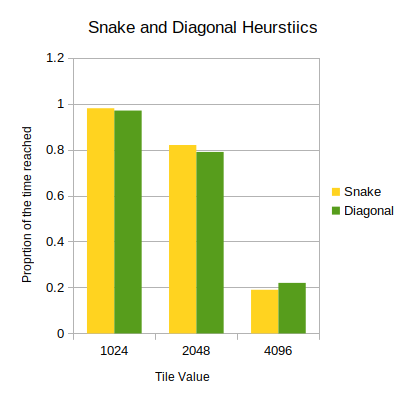
\includegraphics[width=0.4\textwidth]{SnakeToDiagonal.png}
    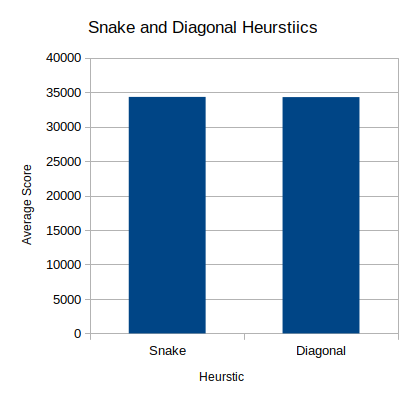
\includegraphics[width=0.4\textwidth]{SnakeToDiagonalScore.png}
    \caption{A compassion between the snake and the diagonal heuristics.}
    \label{fig:SnakeVDiagonal}
\end{figure}


\section{Complexity}
\label{sec:complexity}
\subsection{Time Complexity}
\label{subsec:time_comp}
\subsubsection{$4\times4$ Game}
As the most effective heuristics are currently logged into a $4\times4$ game, I will calculate the time complexity when run on a $4x4$ game, and $n$ is the maximum depth of the tree.

After each maximising node, the tree grows by at most 4. One for each possible move up, down, left and right.

A game starts with two cells; hypothetically, let's say:

\[
\begin{bmatrix}
    2&2&-&-\\
    -&-&-&-\\
    -&-&-&-\\
    -&-&-&-\\
\end{bmatrix}
\]
The best case outcome is that these two cells are merged:
\[
\begin{bmatrix}
    4&-&-&-\\
    -&-&-&-\\
    -&-&-&-\\
    -&-&-&-\\
\end{bmatrix}
\]
This leaves 15 free cells for the new cell to appear; after this, there will be two cells again.
Therefore there can never be more than $15$ free cells.

Therefore the worst case for a chance node has $15\times2=30$ possible outcomes.

For every two layers, the number of leaf nodes multiplies by at most $120$, and there are $n$ layers in the tree.
Therefore Time Complexity To calculate the next move is $120^\frac n 2 = O(\sqrt{120}^n) \approx O(10.954^n)$
\subsubsection{$n \times m$ game}
\subsection{NP Hardness}
\label{subsec:np_hardness}
In a previous paper \cite{LANGERMAN201817}, it has been proven that 2048 is an NP-hard problem...
\newpage
\bibliographystyle{IEEEtran}
\bibliography{refrences}
\end{document}